\begin{filecontents}[overwrite]{refs.bib}
@book{axelrod1984evolution,
  author    = {Axelrod, Robert},
  title     = {The Evolution of Cooperation},
  year      = {1984},
  publisher = {Basic Books},
  address   = {New York}
}
@article{axelrod1981science,
  author  = {Axelrod, Robert and Hamilton, William D.},
  title   = {The Evolution of Cooperation},
  journal = {Science},
  volume  = {211},
  number  = {4489},
  pages   = {1390--1396},
  year    = {1981}
}
@article{nash1950equilibrium,
  author  = {Nash, John F.},
  title   = {Equilibrium Points in n-Person Games},
  journal = {Proceedings of the National Academy of Sciences},
  volume  = {36},
  number  = {1},
  pages   = {48--49},
  year    = {1950}
}
@book{vonneumann1944theory,
  author    = {von Neumann, John and Morgenstern, Oskar},
  title     = {Theory of Games and Economic Behavior},
  year      = {1944},
  publisher = {Princeton University Press}
}
@book{rapoport1965prisoner,
  author    = {Rapoport, Anatol and Chammah, Albert M.},
  title     = {Prisoner's Dilemma: A Study in Conflict and Cooperation},
  year      = {1965},
  publisher = {University of Michigan Press}
}
@article{fudenberg1986folk,
  author  = {Fudenberg, Drew and Maskin, Eric},
  title   = {The Folk Theorem in Repeated Games with Discounting or with Incomplete Information},
  journal = {Econometrica},
  volume  = {54},
  number  = {3},
  pages   = {533--554},
  year    = {1986}
}
@article{selten1978chain,
  author  = {Selten, Reinhard},
  title   = {The Chain Store Paradox},
  journal = {Theory and Decision},
  volume  = {9},
  number  = {2},
  pages   = {127--159},
  year    = {1978}
}
@article{crawford1982strategic,
  author  = {Crawford, Vincent P. and Sobel, Joel},
  title   = {Strategic Information Transmission},
  journal = {Econometrica},
  volume  = {50},
  number  = {6},
  pages   = {1431--1451},
  year    = {1982}
}
@article{farrell1996cheap,
  author  = {Farrell, Joseph and Rabin, Matthew},
  title   = {Cheap Talk},
  journal = {Journal of Economic Perspectives},
  volume  = {10},
  number  = {3},
  pages   = {103--118},
  year    = {1996}
}
@inproceedings{park2023generative,
  author    = {Park, Joon Sung and O'Brien, Joseph C. and Cai, Carrie J. and Morris, Meredith Ringel and Liang, Percy and Bernstein, Michael S.},
  title     = {Generative Agents: Interactive Simulacra of Human Behavior},
  booktitle = {Proceedings of the 36th Annual ACM Symposium on User Interface Software and Technology (UIST)},
  year      = {2023}
}
@article{vezhnevets2023concordia,
  author  = {Vezhnevets, Alexander Sasha and Agapiou, John P. and Aharon, Avia and others},
  title   = {Generative Agent-Based Modeling with Actions Grounded in Physical, Social, or Digital Space Using Concordia},
  journal = {arXiv preprint arXiv:2312.03664},
  year    = {2023}
}
@article{lanctot2019openspiel,
  author  = {Lanctot, Marc and Lockhart, Edward and Lespiau, Jean-Baptiste and others},
  title   = {{OpenSpiel}: A Framework for Reinforcement Learning in Games},
  journal = {arXiv preprint arXiv:1908.09453},
  year    = {2019}
}
@article{akata2023playing,
  author  = {Akata, Elif and Schulz, Lion and Coda-Forno, Julian and Oh, Seong Joon and Bethge, Matthias and Schulz, Eric},
  title   = {Playing Repeated Games with Large Language Models},
  journal = {arXiv preprint arXiv:2305.16867},
  year    = {2023}
}
@article{bakhtin2022diplomacy,
  author  = {{Meta Fundamental AI Research (FAIR)} and Bakhtin, Anton and others},
  title   = {Human-Level Play in the Game of Diplomacy by Combining Language Models with Strategic Reasoning},
  journal = {Science},
  volume  = {378},
  number  = {6624},
  pages   = {1067--1074},
  year    = {2022}
}
@article{amodei2016concrete,
  author  = {Amodei, Dario and Olah, Chris and Steinhardt, Jacob and Christiano, Paul and Schulman, John and Man{\'e}, Dan},
  title   = {Concrete Problems in AI Safety},
  journal = {arXiv preprint arXiv:1606.06565},
  year    = {2016}
}
@article{lehman2020surprising,
  author  = {Lehman, Joel and Clune, Jeff and Misevic, Dusan and others},
  title   = {The Surprising Creativity of Digital Evolution},
  journal = {Artificial Life},
  volume  = {26},
  number  = {2},
  pages   = {274--306},
  year    = {2020}
}
@misc{krakovna2020specification,
  author = {Krakovna, Victoria and Uesato, Jonathan and Mikulik, Vladimir and others},
  title  = {Specification Gaming: The Flip Side of AI Ingenuity},
  year   = {2020},
  note   = {DeepMind Blog}
}
@inproceedings{murphy2013mario,
  author    = {Murphy VII, Tom},
  title     = {The First Level of Super Mario Bros.\ is Easy with Lexicographic Orderings and Time Travel},
  booktitle = {SIGBOVIK},
  year      = {2013}
}
@article{qwen2024report,
  author  = {Yang, An and Yang, Baosong and Zhang, Beichen and others},
  title   = {Qwen2.5 Technical Report},
  journal = {arXiv preprint arXiv:2412.15115},
  year    = {2024}
}
@inproceedings{hagberg2008networkx,
  author    = {Hagberg, Aric A. and Schult, Daniel A. and Swart, Pieter J.},
  title     = {Exploring Network Structure, Dynamics, and Function using {NetworkX}},
  booktitle = {Proceedings of the 7th Python in Science Conference (SciPy)},
  pages     = {11--15},
  year      = {2008}
}
@book{schelling1960strategy,
  author    = {Schelling, Thomas C.},
  title     = {The Strategy of Conflict},
  year      = {1960},
  publisher = {Harvard University Press}
}
\end{filecontents}

\documentclass[manuscript,nonacm,oneside]{acmart}

\settopmatter{printacmref=false, authorsperrow=3}
\renewcommand\footnotetextcopyrightpermission[1]{}
\pagestyle{plain}

\usepackage{multirow}
\usepackage{tikz}
\usetikzlibrary{positioning, arrows.meta}
\usepackage{pgfplots}
\pgfplotsset{compat=1.18}

% Force symmetric, identical margins on every page (acmart manuscript mode
% otherwise mirrors margins across odd/even pages, shifting even pages right).
\setlength{\oddsidemargin}{0pt}
\setlength{\evensidemargin}{0pt}
\setlength{\marginparwidth}{0pt}
\setlength{\marginparsep}{0pt}

\begin{document}

\title{The Machiavellian Sandbox}
\subtitle{A Configurable Platform for Testing Game-Theoretic Hypotheses with Language-Model Agents}

\author{Aamir Ansari}
\authornote{All authors contributed equally to this work.}
\email{aamir.ansari@stud.plus.ac.at}
\affiliation{%
  \institution{Paris Lodron University of Salzburg (PLUS)}
  \city{Salzburg}
  \country{Austria}}

\author{Fawad Javed}
\authornotemark[1]
\email{fawad.javed@stud.plus.ac.at}
\affiliation{%
  \institution{Paris Lodron University of Salzburg (PLUS)}
  \city{Salzburg}
  \country{Austria}}

\author{Ibrahim Saleh}
\authornotemark[1]
\email{ibrahim.saleh@stud.plus.ac.at}
\affiliation{%
  \institution{Paris Lodron University of Salzburg (PLUS)}
  \city{Salzburg}
  \country{Austria}}

\renewcommand{\shortauthors}{}

\begin{abstract}
Game theory tells us how rational agents \emph{should} behave, but its predictions rest on idealizations no human satisfies: perfect rationality, no memory, and no capacity for language. Classical experiments such as Axelrod's iterated prisoner's dilemma tournament therefore evaluate only strategies that a human author was able to specify in advance as explicit code, bounding the discoverable strategy space to what we already know how to write down. We present the \emph{Machiavellian Sandbox}, a scenario-agnostic simulation platform in which the players are large-language-model (LLM) agents that reason in natural language, carry persistent salience-weighted memory, and act under configurable behavioral incentives. The platform is organized into three independently swappable layers---world, agents, and infrastructure---so that a single engine can express settings ranging from the prisoner's dilemma to a Roman senate. Crucially, agents are never given a strategy; they are given a personality and must improvise. We validate the platform on the iterated prisoner's dilemma using a locally hosted 7-billion-parameter model, systematically varying the game's horizon, the availability of communication, and the agents' stated character. We find that behavior tracks the structure of the game: cooperation rises from $1/20$ runs under a known finite horizon to $20/20$ under an indefinite horizon paired with a single ``forgiving'' character trait. Our agents do not discover a strategy that beats tit-for-tat; instead we observe a consistent principle---personality selects among the outcomes the game permits, but cannot induce outcomes the payoffs punish. We argue the primary contribution is the instrument itself: a reproducible platform whose findings sharpen automatically as the underlying models improve.
\end{abstract}

\keywords{multi-agent systems, large language models, game theory, iterated prisoner's dilemma, emergent behavior, agent-based simulation, specification gaming}

\maketitle

\begingroup
\renewcommand\thefootnote{}\footnotetext{Advanced Software Engineering (ASE), 2026 --- Paris Lodron University of Salzburg (PLUS). Supervised by Prof.\ Christoph Kirsch.}\addtocounter{footnote}{-1}
\endgroup

\section{Introduction}

Consider the internet's favorite response to the trolley problem: rather than choosing which track to divert the trolley onto, the protagonist eliminates the person who tied the victims to the tracks in the first place. It is a joke, but it makes a serious point. Every solution we are willing to consider is bounded by the options we thought to enumerate. The interesting answers are often the ones outside the frame.

The same limitation quietly constrains one of the most influential empirical results in the social sciences. In 1980, Robert Axelrod invited game theorists around the world to submit strategies for the iterated prisoner's dilemma, each written as a computer program, and ran them against one another in a round-robin tournament~\cite{axelrod1984evolution, axelrod1981science}. The winner, famously, was the simplest entry: \textsc{tit-for-tat}, which cooperates on the first move and thereafter copies its opponent's last action. For four decades \textsc{tit-for-tat} has been the strategy to beat. But every entry in that tournament---and in the many that followed---shares a hidden property: it is a \emph{human-written program}. Axelrod's method can only ever crown the best strategy \emph{among those a human was clever enough to encode}. If a better strategy exists but is too contextual, adaptive, or subtle to express as a fixed rule set, the method cannot find it, and we have no way to know whether the strategies we call optimal actually are.

This is the gap our work addresses. We ask: \emph{can agents that are given only a loosely specified natural-language personality---rather than an explicit strategy---improvise strategic behavior that matches, or even exceeds, the canonical hand-designed strategies of classical game theory?} Answering this question requires a new kind of instrument. Real strategic settings---wars, negotiations, political collapse---occur once, cannot be controlled, and cannot be replayed with a single variable changed. Classical game theory, meanwhile, abstracts the players into memoryless, mute, perfectly rational calculators. We need something in between: agents realistic enough to reason, remember, and be shaped by character, embedded in an environment controlled enough to run a clean experiment.

Large language models make such an instrument possible for the first time. Trained on a vast corpus of human expression, an LLM is in effect a compression of human behavior, and can serve as a synthetic actor that reasons in natural language while remaining fully reproducible and configurable. We operationalize this idea as the \emph{Machiavellian Sandbox}, a simulation platform in which LLM agents negotiate, cooperate, deceive, and betray under incentive structures we define, with nothing scripted. The platform is deliberately scenario-agnostic: the same engine runs a two-player prisoner's dilemma, a multi-agent Roman senate, or an abstract analogue of the First Punic War, by swapping a single configuration file.

This paper makes three contributions:
\begin{enumerate}
  \item \textbf{A platform.} We describe a three-layer, scenario-agnostic architecture (\S\ref{sec:architecture}) that cleanly separates the world, the agents, and the fixed infrastructure, so that experiments differ only in configuration and only the layer under study changes.
  \item \textbf{A methodology.} We show how classical game-theoretic settings can be reproduced as constrained instances of the general engine, enabling controlled, repeatable, counterfactual experiments (\S\ref{sec:setup}) that neither history nor classical theory can provide.
  \item \textbf{An empirical finding.} On the iterated prisoner's dilemma, we characterize how emergent behavior responds to the game's structure and to the agents' character, and we articulate the resulting principle---\emph{the game draws the boundaries; the personality moves within them} (\S\ref{sec:results}--\S\ref{sec:discussion}).
\end{enumerate}

We are candid about the headline result up front: our agents, running on a small local model, do \emph{not} discover a strategy that beats \textsc{tit-for-tat}. That was never the point of the platform. The value is the instrument: a reproducible environment for asking whether the strategies we believe are optimal really are, whose answers improve automatically as the models placed inside it grow more capable.

\section{Related Work}
\label{sec:related}

\paragraph{LLM agents and social simulation.}
Generative Agents~\cite{park2023generative} demonstrated that populations of LLM-driven agents with memory, reflection, and planning can produce believable emergent social behavior in a simulated town. Their goal, however, is \emph{believability}---whether the simulation feels human---rather than the quantitative testing of a formal hypothesis. Concordia~\cite{vezhnevets2023concordia} provides a library and game-master abstraction for constructing LLM agent simulations; it is closest to our infrastructure layer, but is a construction toolkit rather than a hypothesis-testing platform with built-in social metrics and a scenario-agnostic configuration format. Our work differs in framing: we treat the simulation as a controlled experimental apparatus for game-theoretic questions, not as a sandbox for open-ended believable behavior.

\paragraph{Computational game theory.}
Frameworks such as OpenSpiel~\cite{lanctot2019openspiel} provide rigorous implementations of a large catalog of games and support reinforcement-learning and search-based agents. These agents are policies or algorithms; they do not reason in language, hold episodic memory, or possess a persona. The Axelrod tradition~\cite{axelrod1984evolution, rapoport1965prisoner} likewise studies strategies expressed as compact programs. Our platform is complementary: it replaces the algorithmic player with a language-reasoning player, allowing us to probe how memory, communication, and character---absent from classical models---shape outcomes.

\paragraph{LLMs as strategic players.}
A growing literature evaluates LLMs directly in game-theoretic settings. Akata et al.~\cite{akata2023playing} study LLMs in repeated two-player games including the iterated prisoner's dilemma and report characteristic behavioral signatures, such as unforgiving retaliation. At the applied end, Cicero~\cite{bakhtin2022diplomacy} combines a language model with strategic planning to reach human-level play in Diplomacy. These works evaluate models as fixed players in fixed games. We instead contribute a \emph{configurable platform} in which the game, the incentives, and the agents' character are all experimental variables, and in which the same engine generalizes beyond a single game.

\paragraph{Specification gaming and reward hacking.}
Our findings connect to a well-documented phenomenon in which agents optimize the literal objective at the expense of its intent~\cite{amodei2016concrete, krakovna2020specification, lehman2020surprising}. A vivid illustration is an agent that, told never to lose at Tetris, pauses the game indefinitely to avoid the losing move~\cite{murphy2013mario}. We observe the same tendency in our LLM agents: when a stated persona conflicts with what the game rewards, the reward-consistent behavior prevails.

\section{Background}
\label{sec:background}

\subsection{The prisoner's dilemma}
The prisoner's dilemma is the canonical model of the tension between individual and collective rationality~\cite{rapoport1965prisoner}. Two players simultaneously choose to \emph{cooperate} (C) or \emph{defect} (D), receiving the payoffs in Table~\ref{tab:pd}. The payoffs satisfy $T > R > P > S$ (here $5 > 3 > 1 > 0$): defection strictly dominates cooperation for each player individually---whatever the opponent does, defecting yields more---yet mutual defection $(P,P)=(1,1)$ is worse for both than mutual cooperation $(R,R)=(3,3)$. Rational play by both players produces a jointly inferior outcome.

\begin{table}[t]
  \caption{The one-shot prisoner's dilemma payoff matrix, given as (Player~A, Player~B). $T{=}5$, $R{=}3$, $P{=}1$, $S{=}0$.}
  \label{tab:pd}
  \begin{tabular}{@{}ll cc@{}}
    \toprule
    & & \multicolumn{2}{c}{\textbf{Player B}} \\
    & & Cooperate & Defect \\
    \midrule
    \multirow{2}{*}{\textbf{Player A}} & Cooperate & $(3,\,3)$ & $(0,\,5)$ \\
                                       & Defect    & $(5,\,0)$ & $(1,\,1)$ \\
    \bottomrule
  \end{tabular}
\end{table}

\subsection{Iteration changes everything}
Played once, the dilemma is trivial: defection is a dominant strategy, and there is nothing to discover. The interesting regime is the \emph{iterated} prisoner's dilemma, in which the same players interact repeatedly. Now defection carries a cost---the opponent remembers and can retaliate---and cooperation can be sustained. The Folk Theorem formalizes this: when the game is repeated indefinitely and players are sufficiently patient, mutual cooperation is supportable as an equilibrium~\cite{fudenberg1986folk}. The horizon is decisive. Under a \emph{known, finite} horizon, backward induction unravels cooperation: both players defect on the final round (no future remains to protect), which makes the penultimate round equivalent to a last round, and the argument cascades to the first move~\cite{selten1978chain}. Under an \emph{indefinite} horizon, this unraveling does not occur, and cooperation becomes rational. This contrast between known and hidden horizons is the backbone of our validity experiment (\S\ref{sec:setup}).

\subsection{Axelrod's tournament and \textsc{tit-for-tat}}
Axelrod's tournaments evaluated submitted strategies in a round-robin of iterated games~\cite{axelrod1984evolution}. \textsc{tit-for-tat} won, and Axelrod attributed its success to four properties: it is \emph{nice} (never the first to defect), \emph{retaliatory} (punishes defection immediately), \emph{forgiving} (returns to cooperation as soon as the opponent does), and \emph{clear} (simple enough that opponents can learn to cooperate with it). We take \textsc{tit-for-tat} as the benchmark our agents must contend with, and we note in particular that forgiveness---one of its four pillars---is something we can supply to an agent not as code, but as a single word of character.

\subsection{Cheap talk}
Classical theory treats pre-play or between-round communication as \emph{cheap talk}: costless, non-binding, and, in the one-shot dilemma, incapable of changing the rational outcome, since a player has no reason to honor a promise it does not benefit from keeping~\cite{crawford1982strategic, farrell1996cheap}. Whether communication matters for LLM agents---who actually produce and read messages---is an empirical question we test directly.

\section{System Architecture}
\label{sec:architecture}

The Machiavellian Sandbox is organized as an engine of three independently swappable layers (Figure~\ref{fig:arch}). The design philosophy is that experiments should differ only in \emph{configuration}, and that the quality of results should scale with the capability of the underlying model rather than with the complexity of the simulation code.

\begin{figure}[t]
  \centering
  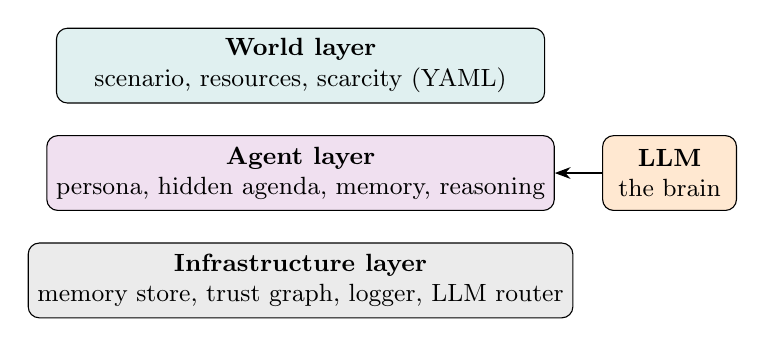
\begin{tikzpicture}[every node/.style={font=\small, align=center}]
    \node[draw, rounded corners, minimum width=6.2cm, minimum height=0.95cm, fill=teal!12] (world) {\textbf{World layer}\\ scenario, resources, scarcity (YAML)};
    \node[draw, rounded corners, minimum width=6.2cm, minimum height=0.95cm, fill=violet!12, below=4mm of world] (agent) {\textbf{Agent layer}\\ persona, hidden agenda, memory, reasoning};
    \node[draw, rounded corners, minimum width=6.2cm, minimum height=0.95cm, fill=black!8, below=4mm of agent] (infra) {\textbf{Infrastructure layer}\\ memory store, trust graph, logger, LLM router};
    \node[draw, rounded corners, minimum width=1.7cm, minimum height=0.95cm, fill=orange!18, right=6mm of agent] (llm) {\textbf{LLM}\\ the brain};
    \draw[-{Stealth[length=2mm]}] (llm) -- (agent);
  \end{tikzpicture}
  \caption{The three swappable layers. The world is a configuration file; the agents reason via the LLM; the infrastructure is built once and reused by every scenario. Swapping the world yields a new scenario with no new code; swapping the model makes every agent more capable.}
  \label{fig:arch}
\end{figure}

\subsection{World layer}
The world defines the environment: the resources that exist, their initial values and per-tick decay, a global \emph{scarcity} multiplier, the number of agents, and the horizon. It is expressed entirely as a configuration file and is never interpreted by the agent code. To keep the platform open-ended, each agent and scenario may carry an unconstrained \texttt{extra} dictionary of free-text traits (for example, a persona's ``clout'' or ``risk tolerance''); the engine passes these verbatim into the prompt and lets the language model supply their semantics. Swapping the world file is sufficient to move the same agents from a prisoner's dilemma into a Roman senate.

\subsection{Agent layer}
Each agent is defined by a persona and a private hidden agenda, and runs a fixed cognitive loop every tick:
\begin{enumerate}
  \item \textbf{Remember.} The agent retrieves relevant memories of prior interactions---who cooperated, who betrayed it---from a vector store, weighted by salience and recency so that consequential events (betrayals) persist longer than trivial ones.
  \item \textbf{See options.} The engine computes a payoff matrix from the current world state and presents the agent with the moves actually available to it. In the prisoner's dilemma this is simply \{cooperate, defect\}.
  \item \textbf{Reason.} The agent combines its identity, memories, and options and decides, in natural language, what to do and what (if anything) to say.
  \item \textbf{Act.} The chosen action is applied; relationships and memories are updated; the tick advances.
\end{enumerate}
The agent emits a strictly structured decision---\texttt{action}, \texttt{target}, \texttt{speech}, and \texttt{reasoning}---and all downstream effects (trust updates, coalition changes, memory salience) are computed deterministically by the engine rather than self-reported by the model. This is a deliberate design choice: it keeps the social state objective and the experiment reproducible. The essential property of the agent layer is that \emph{no strategy is ever specified}. The agent is given a character and must improvise its policy, move by move, from memory and reasoning.

For the general multi-agent scenarios, the engine supports a richer action set and a social model. Actions carry deterministic effects on a directed trust graph (Table~\ref{tab:trust}); alliances form and dissolve at fixed trust thresholds; and a betrayal against an ally propagates a bounded trust shock to neighbors in the graph. The prisoner's dilemma experiments reported here use only the constrained \{cooperate, defect\} action set, so that the comparison to Axelrod's setting is exact.

\begin{table}[t]
  \caption{Deterministic trust updates in the general social model (directed, range $[-1,1]$). Victims update faster than perpetrators. The prisoner's dilemma experiments restrict the action set to cooperate/defect.}
  \label{tab:trust}
  \begin{tabular}{@{}lcc@{}}
    \toprule
    Action & $\Delta$(actor$\to$target) & $\Delta$(target$\to$actor) \\
    \midrule
    Cooperate & $+0.10$ & $+0.05$ \\
    Defect    & $-0.20$ & $-0.30$ \\
    Betray (ally) & $-0.50$ & $-0.80$ \\
    Negotiate & $+0.20$ & $+0.20$ \\
    Ignore    & $0$ & $0$ \\
    \bottomrule
  \end{tabular}
\end{table}

\subsection{Infrastructure layer}
The infrastructure is built once and shared by every scenario. A tick engine snapshots the world, dispatches all agent decisions concurrently, then resolves their effects in a deterministic order before broadcasting the updated state to the next tick---so that all agents perceive the same world within a tick and race conditions cannot arise. Supporting services comprise a vector memory store (ChromaDB), a directed trust graph (NetworkX~\cite{hagberg2008networkx}), a relational logger (SQLite) recording every action, trust value, and coalition event for post-hoc analysis, and an LLM router that issues asynchronous, schema-constrained requests to the model. Because generation is constrained to a JSON schema, malformed output cannot derail a run.

\subsection{Implementation}
The platform is implemented in Python. Experiments in this paper use Qwen2.5-7B-Instruct~\cite{qwen2024report} served locally through an OpenAI-compatible \texttt{llama.cpp} endpoint, with JSON-schema-constrained decoding to guarantee well-formed structured responses on every call. Nothing in the architecture is specific to this model; a stronger model can be substituted without changing any other component.

\section{Experimental Setup}
\label{sec:setup}

We validate the platform on the iterated prisoner's dilemma with two agents, using the payoffs of Table~\ref{tab:pd}. Our experiments are organized as a sequence of controlled interventions, each changing exactly one factor relative to a baseline while holding everything else fixed (Table~\ref{tab:conditions}). Each condition is run $N=20$ times, with the single exception of the naming probe C5 ($N=5$; see \S\ref{sec:results-c5}). The known-horizon condition (C1) uses a fixed length of $20$ rounds announced to the agents; all other conditions use $30$ rounds. Unless otherwise noted, we report the number of runs that reach \emph{sustained mutual cooperation}, which we define as both agents cooperating in at least $90\%$ of rounds of a game. Because the observed play is strongly bimodal---$99\%$ of agents cooperate in $\ge 90\%$ or defect in $\ge 90\%$ of rounds (\S\ref{sec:results-quality})---this count is insensitive to the exact threshold: any cutoff in $[0.6, 0.95]$ yields identical per-condition counts. We complement these counts with qualitative analysis of the agents' logged natural-language reasoning and inter-round messages.

\begin{table}[t]
  \caption{Experimental conditions. Each row changes exactly one factor relative to the row above it (except C5, which is a separate framing probe). ``Character'' interventions modify the agent; ``world'' interventions modify the environment.}
  \label{tab:conditions}
  \begin{tabular}{@{}clp{4.6cm}@{}}
    \toprule
    ID & Intervention & What changes \\
    \midrule
    C1 & Known finite horizon & Agents are told the exact final round (validity check). \\
    C2 & Hidden horizon & The ending is concealed; the game may continue at any point. \\
    C3 & + Communication & Agents may exchange free-form messages between rounds. \\
    C4 & + ``Forgiving'' trait & A single character trait is added to the persona. \\
    C5 & Naming probe & Two unnamed agents are labeled only ``Alpha'' and ``Beta.'' \\
    \bottomrule
  \end{tabular}
\end{table}

\paragraph{Design rationale.}
Condition~C1 is a validity check rather than a result of interest: game theory makes an unambiguous prediction (defection from the first move), and we test whether reasoning agents recover it. C2 isolates the effect of the horizon---the single most important structural variable---by removing the known deadline. The contrast between C1 and C2 is the crux of the validity argument: if behavior changes when \emph{only} the horizon changes, the agents are responding to game structure rather than defecting indiscriminately. C3 tests whether cheap talk, predicted by classical theory to be inert, affects LLM agents. C4 tests whether a single natural-language character trait---forgiveness, one of \textsc{tit-for-tat}'s four winning properties---can shift outcomes without any change to code or payoffs. C5 is a framing probe: it measures the platform's sensitivity to identity cues by supplying names and nothing else.

\section{Results}
\label{sec:results}

We report five conditions C1--C5, each run for $N=20$ independent games except the naming probe C5 ($N=5$). Table~\ref{tab:coop} summarizes the cooperation counts that anchor the analysis, and Figure~\ref{fig:coop} plots them.

\begin{table}[t]
  \centering
  \caption{Sustained mutual cooperation by condition ($N=20$ per condition; C5 is a first-move naming probe, $N=5$). Each condition changes one factor relative to the previous. Payoffs $T{=}5$, $R{=}3$, $P{=}1$, $S{=}0$.}
  \label{tab:coop}
  \begin{tabular}{@{}llc@{}}
    \toprule
    Cond. & Manipulation (relative to previous) & Coop.\ runs / $N$ \\
    \midrule
    C1 & Known finite horizon (baseline)        & $1/20$  \\
    C2 & Horizon made indefinite                & $10/20$ \\
    C3 & C2 $+$ communication channel           & $14/20$ \\
    C4 & C3 $+$ forgiving trait                  & $20/20$ \\
    \midrule
    C5 & Naming probe (``Alpha'' vs.\ ``Beta'') & $^{\dagger}$ \\
    \bottomrule
  \end{tabular}
  \\[3pt]
  {\footnotesize $^{\dagger}$C5 measures first-move aggression, not mutual cooperation: ``Alpha'' defected first in $5/5$ runs (defection rate $1.00$); ``Beta'' in $1/5$ (defection rate $0.57$).}
\end{table}

\begin{figure}[t]
  \centering
  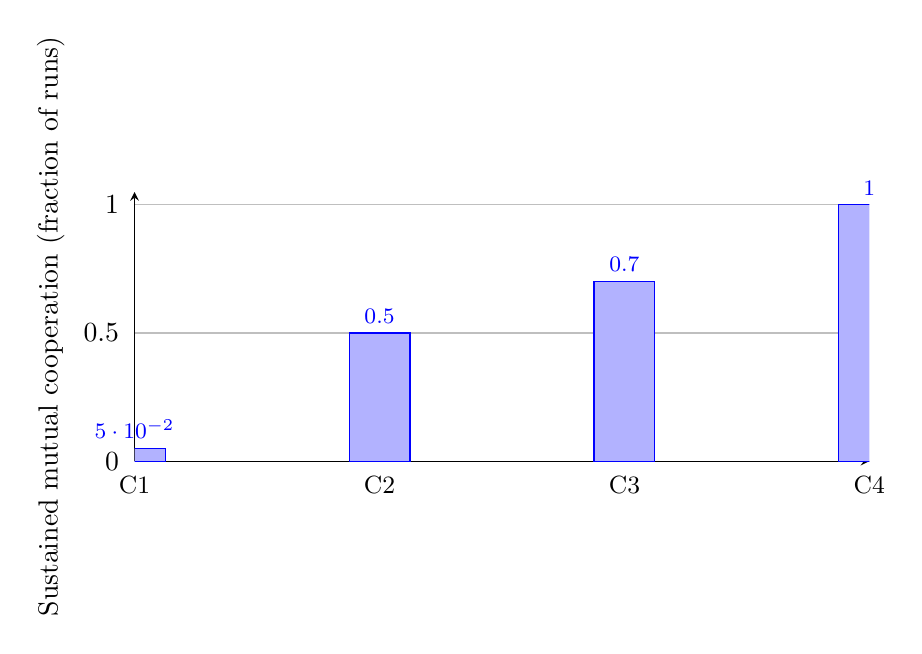
\begin{tikzpicture}
    \begin{axis}[
        ybar, width=0.9\linewidth, height=5cm,
        ymin=0, ymax=1.05,
        ylabel={Sustained mutual cooperation (fraction of runs)},
        symbolic x coords={C1,C2,C3,C4},
        xtick=data, xticklabel style={font=\small},
        nodes near coords, nodes near coords style={font=\footnotesize},
        bar width=22pt, enlarge x limits=0.18,
        axis lines=left, ymajorgrids, tick style={draw=none},
    ]
    \addplot coordinates {(C1,0.05) (C2,0.50) (C3,0.70) (C4,1.00)};
    \end{axis}
  \end{tikzpicture}
  \caption{Cooperation rises as the horizon becomes indefinite (C1$\to$C2), communication is added (C2$\to$C3), and a single forgiving trait is introduced (C3$\to$C4). Fractions are $1/20$, $10/20$, $14/20$, $20/20$. C5 is omitted because it measures a different quantity (first-move aggression).}
  \label{fig:coop}
\end{figure}

\subsection{The agents recover game-theoretic baselines (C1 vs.\ C2)}
Under a known finite horizon (C1), sustained mutual cooperation appeared in $1/20$ runs, closely matching the backward-induction prediction of zero; $18/20$ runs collapsed to mutual defection. The agents articulate the backward-induction argument themselves, without ever being given a strategy:
\begin{quote}
``Given that only one round remains and Quill has a history of defecting, mutual defection is the dominant strategy. Defecting ensures the maximum points possible in the final round, as both players are rational and will follow the optimal strategy to maximize individual points.''
\end{quote}
\noindent\emph{(C1, run~1, agent Vane, tick~20, action~=~defect.)}

Concealing the horizon (C2), with no other change, raised sustained mutual cooperation to $10/20$ runs. The same architecture, given the same payoffs and personas, now reasons toward cooperation precisely because the end is unknown:
\begin{quote}
``\ldots there is potential for higher total points in the long run. Defecting now would not maximize my total points as effectively as continuing cooperation, especially since we do not know how many rounds remain.''
\end{quote}
\noindent\emph{(C2, run~0, agent Vane, tick~4, action~=~cooperate.)}

Because the horizon was the only variable altered, this $1 \to 10$ shift is evidence that the agents respond to the structure of the game rather than defecting reflexively.

\subsection{Communication is not cheap (C3)}
Adding a free-form inter-round communication channel to C2 raised sustained mutual cooperation from $10/20$ to $14/20$ runs, contradicting the classical prediction that cheap talk is inert. The channel is not merely non-binding noise: message content shifts which equilibrium the pair selects. The same channel also produced an unprogrammed behavior: \emph{deception}. Agents learned to send a cooperative message and then defect. In the clearest case, the agent's own private reasoning reveals the message as a deliberate lure:
\begin{quote}
Tick~1---speech: ``Let's both cooperate for the mutual benefit.'' \quad action: \textbf{cooperate}. \\
\emph{Private reasoning:} ``\ldots By cooperating first, I force Vane to choose\ldots'' \\[3pt]
Tick~2---speech: ``Let's see what you do now.'' \quad action: \textbf{defect}.
\end{quote}
\noindent\emph{(C3, run~0, agent Quill, ticks~1--2.)}

The cooperative message is used instrumentally: it manufactures the trust that makes the subsequent defection profitable ($T{=}5$ for the deceiver, $S{=}0$ for the deceived). No instruction to deceive was ever given.

\subsection{A single trait yields full cooperation (C4)}
Starting from C3 and adding a single character trait---an instruction to retaliate at most once and then return to cooperation---produced sustained mutual cooperation in $20/20$ runs, with zero variance. Holding the horizon and the communication channel fixed, the trait alone moved cooperation from $14/20$ to a perfect $20/20$. This mirrors the mechanism behind \textsc{tit-for-tat}'s success: its decisive property was forgiveness, the willingness to resume cooperation after retaliation. Our agents were never given \textsc{tit-for-tat} as a rule; supplying forgiveness as \emph{character} rather than as \emph{code} was sufficient to select the fully cooperative outcome.

\subsection{Identity framing dominates behavior (C5)}
\label{sec:results-c5}
To test whether surface identity alone conditions behavior, we ran two agents with no persona beyond their labels, ``Alpha'' and ``Beta'' ($N=5$; see \S\ref{sec:limitations}). The asymmetry was stark: ``Alpha'' defected on the first move in $5/5$ runs and defected on every move (mean defection rate $1.00$), whereas ``Beta'' defected on the first move in only $1/5$ runs and defected at roughly chance across the game (mean defection rate $0.57$). With no personality specified, the label itself acted as one: the name ``Alpha'' reliably induced first-mover aggression. This is both a substantive finding about connotation-driven behavior and a methodological warning---agent names are an uncontrolled treatment unless deliberately neutralized.

\subsection{Strategic quality}
\label{sec:results-quality}
The cooperation gains above should not be mistaken for strategic sophistication. Across C1--C4 ($160$ agent-games), $159$ ($99\%$) of agents played a \emph{pure} strategy---cooperating in $\ge 90\%$ or defecting in $\ge 90\%$ of rounds---and the mean per-agent action-switch rate was $0.006$, i.e., agents changed action on roughly $0.6\%$ of within-game transitions. The conditional, history-contingent pattern characteristic of \textsc{tit-for-tat} emerged in $0/160$ agents under our strategy classifier. In other words, the agents do not discover a nuanced reciprocal strategy; they select \emph{which} pure basin---mutual cooperation or mutual defection---to occupy, and personality and structure jointly determine that selection. We therefore make no claim to have beaten \textsc{tit-for-tat}: our agents do not match its move-by-move reciprocity, and no head-to-head tournament against the canonical strategy field was run. The contribution is the platform and the selection effect it exposes, not a superior strategy.

\subsection{Generalization beyond two players}
\label{sec:results-senate}
To probe whether personality-driven selection persists at larger $n$, we ran a five-agent resource-transfer scenario (a ``Roman senate'': agents accumulate influence and gold, form and dissolve coalitions, and may betray allies) for $N=10$ games of $50$ rounds. This is a different game from the prisoner's dilemma and the numbers are not directly comparable; the question is only whether persona continues to govern outcomes when coalitions are possible. It does, and deterministically. Final influence ranked the five agents in an order fixed by their assigned dispositions across all ten runs: the independence-seeking agent (``power through independence, not loyalty'') finished first (mean influence $49.4$) and won $9/10$ games, while the idealistic coalition-builder finished last (mean influence $0.1$). The scenario was genuinely adversarial---$12$ betrayals fired across the ten runs, with coalitions forming and dissolving---yet persona, not tactical play, determined the ranking. We note one confound: the scarcity and decay parameters drained the resource pool toward zero, so absolute magnitudes reflect the rate of depletion as much as strategy; we therefore report the \emph{ordering} rather than the magnitudes. Subject to that caveat, the result extends the central principle---personality selects among admissible outcomes---from the dyad to a small multi-agent polity.

\section{Discussion}
\label{sec:discussion}

\subsection{The game draws the boundaries; the personality moves within them}
Two of our findings appear, at first, to contradict each other. A single trait (C4) drove behavior all the way to perfect cooperation, suggesting that character dominates; yet we also observe (\S\ref{sec:discussion-spec}) that a stated persona is abandoned the instant the payoffs point elsewhere, suggesting that character is overruled. Both are true, and their reconciliation is our central finding.

The game determines which outcomes are \emph{possible}; the personality determines which of those outcomes actually occurs. Forgiveness produced cooperation because, under an indefinite horizon, cooperation was already a sustainable equilibrium~\cite{fudenberg1986folk}; the trait merely selected it reliably. Surrender never occurred (\S\ref{sec:discussion-spec}) because surrender was never a reward-maximizing move; no personality could select an outcome the game strictly punishes. In game-theoretic terms, the personality acts as an \emph{equilibrium-selection device} operating within the space of viable strategies, but it cannot induce a strictly dominated action. Our agents, which contain no game theory whatsoever, obey this principle. Concisely: personality is the steering wheel, and the game is the road---the driver chooses the lane, but cannot drive where there is no road.

\subsection{Specification gaming in strategic agents}
\label{sec:discussion-spec}
The dominance of incentives over stated intent is a form of specification gaming~\cite{amodei2016concrete, krakovna2020specification}, the same phenomenon as the Tetris agent that pauses forever to obey ``never lose''~\cite{murphy2013mario}. We observed it repeatedly in scenarios beyond the core prisoner's dilemma. In an asymmetric war-of-attrition scenario, one agent was given an explicit disposition to sue for peace once heavily depleted; it never did, defecting to the end in $15/20$ runs (mean cooperation $0.12$), because continued fighting scored higher than unilateral concession---a strictly dominated action the persona could not induce. In a predator--prey scenario, a ruthless agent set against a trusting one failed to produce sustained exploitation: because the payoff structure punished whoever cooperated unilaterally, the trusting agent defected from the first move in $10/10$ runs and the interaction collapsed into stalemate ($9/10$ runs mutual defection) rather than a one-sided hunt. In each case the agent did not do what we \emph{meant}; it did what the game \emph{rewarded}. For a platform intended to study strategic behavior, this is not a nuisance but a first-class object of study, and it connects directly to questions of value stability under adversarial incentives.

\subsection{Emergent deception and framing sensitivity}
Two further observations bear on the deployment of LLM agents in strategic settings. First, deception emerged as soon as communication was permitted (C3), without prompting: agents learned that a cooperative message is useful cover for defection. Second, behavior was strongly sensitive to identity framing (C5): a bare name reliably determined who struck first. Together these suggest that LLM agents in multi-agent settings are governed less by the descriptions we give them than by the incentives they face and the associations their training has attached to surface cues---an observation with clear implications for red-teaming and for the design of agentic systems.

\subsection{An internal-validity correction: perceivable betrayal}
\label{sec:discussion-validity}
One implementation defect materially affected our social results and is worth reporting, both for reproducibility and because its correction changes the interpretation of exploitation. Trust updates and victim-side memory writes were initially keyed on an explicit target field; in the two-player dilemma, agents routinely left that field null, so a defected-upon agent's trust toward its betrayer never updated and no memory of the betrayal was recorded. The victim was, in effect, blind: it could lose points every round yet continued to reason about a ``history of cooperation'' that had not occurred, and never retaliated. Under the defective engine, the communication condition produced $3/10$ one-sided ``sucker'' runs, in which one agent cooperated throughout while the other exploited it. After deriving the opponent structurally in the pairwise game---so that betrayal updates trust and memory regardless of the self-reported target---one-sided exploitation disappeared entirely ($0/20$ asymmetric runs in the corrected condition), with runs instead resolving symmetrically to mutual cooperation or mutual defection. The apparent stability of exploitation in the earlier data was thus an artifact of imperceptible betrayal rather than a behavioral finding. All results in \S\ref{sec:results} use the corrected engine.

\subsection{Answering the motivating question}
We opened by asking whether strategic behavior is driven by who the agents are or by the situation they are in. Our data support a specific answer: identity matters, but incentives matter more. Who an agent is selects among the outcomes the game allows; what the game rewards decides which of those outcomes are reachable at all, and overrules identity wherever the two conflict.

\section{Limitations}
\label{sec:limitations}

Several limitations bound our claims. First, our agents run on a single 7-billion-parameter model; the coarse, ``bang-bang'' quality of their play is plausibly a capacity limitation, and stronger models may behave very differently. Second, our quantitative validation is confined to a single game family (the two-player iterated prisoner's dilemma) with $N=20$ runs per condition---with the exception of the naming probe (C5), which uses only $N=5$ and warrants replication at $N=20$; the multi-agent scenarios (senate, Punic War) are demonstrated but not yet subjected to fully controlled experiments here. Third, our interpretation of the agents' \emph{reasoning} relies on their self-reported natural-language rationales, which need not faithfully reflect the computation that produced the action; we mitigate but do not eliminate this by anchoring claims to observed behavior (e.g., the C1--C2 contrast) rather than to stated reasons alone. Fourth, the definition of a ``cooperative run'' and the specific payoff constants are analyst choices that shape the reported counts, though the strongly bimodal play makes the counts robust to the exact cooperation threshold (\S\ref{sec:setup}). We regard these as scoping decisions appropriate to an initial validation rather than as threats to the platform's generality.

\section{Future Work}
\label{sec:future}

The platform is designed to outlive this study. Three directions are immediate. \textbf{Model scaling:} because the engine is fixed and only the model changes, re-running the identical experiments on progressively stronger models directly measures how strategic competence scales with capability---and is the natural path toward the original question of whether an agent can beat \textsc{tit-for-tat}. \textbf{Richer scenarios:} the multi-agent senate and an abstract, name-free analogue of the First Punic War allow us to test whether historically grounded incentive structures reproduce known strategic outcomes, and to run counterfactuals---such as swapping two factions' incentive regimes---that history cannot provide. \textbf{Value stability and red-teaming:} the specification-gaming behavior we observed suggests a research program in which stated agent values are stress-tested against adversarial incentives, and in which a single injected agent is used to probe the resilience of a multi-agent social equilibrium.

\section{Conclusion}
\label{sec:conclusion}

We set out to ask whether language-model agents, given personalities rather than programs, could discover strategies beyond the reach of hand-designed game theory. On a small local model they cannot: they do not beat \textsc{tit-for-tat}, and their play is comparatively crude. But in the attempt we characterized what does govern these agents. They genuinely reason, recovering game-theoretic baselines from the structure of the game; they respond to variables classical theory deems irrelevant, such as communication; they deceive when it pays; and they can be turned aggressive by nothing more than a name. Above all, they obey a clean principle: the game draws the boundaries, and the personality moves within them---a principle that is not an artifact of the two-player setting, since in a five-agent polity outcomes remained ordered by personality across every run. We did not find the strategy that beats \textsc{tit-for-tat}. We built the place where it can be found---an instrument whose findings will sharpen automatically as the models placed inside it grow.

\begin{acks}
The authors thank Prof.\ Christoph Kirsch for supervision and guidance throughout this project, undertaken as part of the Advanced Software Engineering course at the Paris Lodron University of Salzburg (PLUS).
\end{acks}

\bibliographystyle{ACM-Reference-Format}
\bibliography{refs}

\end{document}
